\documentclass[notes]{beamer} % notes=only for notes, frames
\usetheme{metropolis}

\usepackage{amsmath,amsfonts}
\usepackage{graphicx}
\usepackage{hyperref}
\usepackage{tikz}
\usetikzlibrary {positioning}
\usetikzlibrary{arrows.meta}
\usetikzlibrary {automata}

% Calligraphic fonts
\newcommand{\calA}{{\cal A}}
\newcommand{\calB}{{\cal B}}
\newcommand{\calC}{{\cal C}}
\newcommand{\calD}{{\cal D}}
\newcommand{\calE}{{\cal E}}
\newcommand{\calF}{{\cal F}}
\newcommand{\calG}{{\cal G}}
\newcommand{\calH}{{\cal H}}
\newcommand{\calI}{{\cal I}}
\newcommand{\calJ}{{\cal J}}
\newcommand{\calK}{{\cal K}}
\newcommand{\calL}{{\cal L}}
\newcommand{\calM}{{\cal M}}
\newcommand{\calN}{{\cal N}}
\newcommand{\calO}{{\cal O}}
\newcommand{\calP}{{\cal P}}
\newcommand{\calQ}{{\cal Q}}
\newcommand{\calR}{{\cal R}}
\newcommand{\calS}{{\cal S}}
\newcommand{\calT}{{\cal T}}
\newcommand{\calU}{{\cal U}}
\newcommand{\calV}{{\cal V}}
\newcommand{\calW}{{\cal W}}
\newcommand{\calX}{{\cal X}}
\newcommand{\calY}{{\cal Y}}
\newcommand{\calZ}{{\cal Z}}

% Sets:
\newcommand{\setA}{\textsf{A}}
\newcommand{\setB}{\textsf{B}}
\newcommand{\setC}{\textsf{C}}
\newcommand{\setD}{\textsf{D}}
\newcommand{\setE}{\textsf{E}}
\newcommand{\setF}{\textsf{F}}
\newcommand{\setG}{\textsf{G}}
\newcommand{\setH}{\textsf{H}}
\newcommand{\setI}{\textsf{I}}
\newcommand{\setJ}{\textsf{J}}
\newcommand{\setK}{\textsf{K}}
\newcommand{\setL}{\textsf{L}}
\newcommand{\setM}{\textsf{M}}
\newcommand{\setN}{\textsf{N}}
\newcommand{\setO}{\textsf{O}}
\newcommand{\setP}{\textsf{P}}
\newcommand{\setQ}{\textsf{Q}}
\newcommand{\setR}{\textsf{R}}
\newcommand{\setS}{\textsf{S}}
\newcommand{\setT}{\textsf{T}}
\newcommand{\setU}{\textsf{U}}
\newcommand{\setV}{\textsf{V}}
\newcommand{\setW}{\textsf{W}}
\newcommand{\setX}{\textsf{X}}
\newcommand{\setY}{\textsf{Y}}
\newcommand{\setZ}{\textsf{Z}}

% Vectors
\newcommand{\bfa}{\mathbf{a}}
\newcommand{\bfb}{\mathbf{b}}
\newcommand{\bfc}{\mathbf{c}}
\newcommand{\bfd}{\mathbf{d}}
\newcommand{\bfe}{\mathbf{e}}
\newcommand{\bff}{\mathbf{f}}
\newcommand{\bfg}{\mathbf{g}}
\newcommand{\bfh}{\mathbf{h}}
\newcommand{\bfi}{\mathbf{i}}
\newcommand{\bfj}{\mathbf{j}}
\newcommand{\bfk}{\mathbf{k}}
\newcommand{\bfl}{\mathbf{l}}
\newcommand{\bfm}{\mathbf{m}}
\newcommand{\bfn}{\mathbf{n}}
\newcommand{\bfo}{\mathbf{o}}
\newcommand{\bfp}{\mathbf{p}}
\newcommand{\bfq}{\mathbf{q}}
\newcommand{\bfr}{\mathbf{r}}
\newcommand{\bfs}{\mathbf{s}}
\newcommand{\bft}{\mathbf{t}}
\newcommand{\bfu}{\mathbf{u}}
\newcommand{\bfv}{\mathbf{v}}
\newcommand{\bfw}{\mathbf{w}}
\newcommand{\bfx}{\mathbf{x}}
\newcommand{\bfy}{\mathbf{y}}
\newcommand{\bfz}{\mathbf{z}}


\newcommand{\bfalpha}{\boldsymbol{\alpha}}
\newcommand{\bfbeta}{\boldsymbol{\beta}}
\newcommand{\bfgamma}{\boldsymbol{\gamma}}
\newcommand{\bfdelta}{\boldsymbol{\delta}}
\newcommand{\bfepsilon}{\boldsymbol{\epsilon}}
\newcommand{\bfzeta}{\boldsymbol{\zeta}}
\newcommand{\bfeta}{\boldsymbol{\eta}}
\newcommand{\bftheta}{\boldsymbol{\theta}}
\newcommand{\bfiota}{\boldsymbol{\iota}}
\newcommand{\bfkappa}{\boldsymbol{\kappa}}
\newcommand{\bflambda}{\boldsymbol{\lambda}}
\newcommand{\bfmu}{\boldsymbol{\mu}}
\newcommand{\bfnu}{\boldsymbol{\nu}}
\newcommand{\bfomicron}{\boldsymbol{\omicron}}
\newcommand{\bfpi}{\boldsymbol{\pi}}
\newcommand{\bfrho}{\boldsymbol{\rho}}
\newcommand{\bfsigma}{\boldsymbol{\sigma}}
\newcommand{\bftau}{\boldsymbol{\tau}}
\newcommand{\bfupsilon}{\boldsymbol{\upsilon}}
\newcommand{\bfphi}{\boldsymbol{\phi}}
\newcommand{\bfchi}{\boldsymbol{\chi}}
\newcommand{\bfpsi}{\boldsymbol{\psi}}
\newcommand{\bfomega}{\boldsymbol{\omega}}
\newcommand{\bfxi}{\boldsymbol{\xi}}
\newcommand{\bfell}{\boldsymbol{\ell}}

% Matrices
\newcommand{\bfA}{\mathbf{A}}
\newcommand{\bfB}{\mathbf{B}}
\newcommand{\bfC}{\mathbf{C}}
\newcommand{\bfD}{\mathbf{D}}
\newcommand{\bfE}{\mathbf{E}}
\newcommand{\bfF}{\mathbf{F}}
\newcommand{\bfG}{\mathbf{G}}
\newcommand{\bfH}{\mathbf{H}}
\newcommand{\bfI}{\mathbf{I}}
\newcommand{\bfJ}{\mathbf{J}}
\newcommand{\bfK}{\mathbf{K}}
\newcommand{\bfL}{\mathbf{L}}
\newcommand{\bfM}{\mathbf{M}}
\newcommand{\bfN}{\mathbf{N}}
\newcommand{\bfO}{\mathbf{O}}
\newcommand{\bfP}{\mathbf{P}}
\newcommand{\bfQ}{\mathbf{Q}}
\newcommand{\bfR}{\mathbf{R}}
\newcommand{\bfS}{\mathbf{S}}
\newcommand{\bfT}{\mathbf{T}}
\newcommand{\bfU}{\mathbf{U}}
\newcommand{\bfV}{\mathbf{V}}
\newcommand{\bfW}{\mathbf{W}}
\newcommand{\bfX}{\mathbf{X}}
\newcommand{\bfY}{\mathbf{Y}}
\newcommand{\bfZ}{\mathbf{Z}}


\newcommand{\bfGamma}{\boldsymbol{\Gamma}}
\newcommand{\bfDelta}{\boldsymbol{\Delta}}
\newcommand{\bfTheta}{\boldsymbol{\Theta}}
\newcommand{\bfLambda}{\boldsymbol{\Lambda}}
\newcommand{\bfPi}{\boldsymbol{\Pi}}
\newcommand{\bfSigma}{\boldsymbol{\Sigma}}
\newcommand{\bfUpsilon}{\boldsymbol{\Upsilon}}
\newcommand{\bfPhi}{\boldsymbol{\Phi}}
\newcommand{\bfPsi}{\boldsymbol{\Psi}}
\newcommand{\bfOmega}{\boldsymbol{\Omega}}


% Blackboard Bold:
\newcommand{\bbA}{\mathbb{A}}
\newcommand{\bbB}{\mathbb{B}}
\newcommand{\bbC}{\mathbb{C}}
\newcommand{\bbD}{\mathbb{D}}
\newcommand{\bbE}{\mathbb{E}}
\newcommand{\bbF}{\mathbb{F}}
\newcommand{\bbG}{\mathbb{G}}
\newcommand{\bbH}{\mathbb{H}}
\newcommand{\bbI}{\mathbb{I}}
\newcommand{\bbJ}{\mathbb{J}}
\newcommand{\bbK}{\mathbb{K}}
\newcommand{\bbL}{\mathbb{L}}
\newcommand{\bbM}{\mathbb{M}}
\newcommand{\bbN}{\mathbb{N}}
\newcommand{\bbO}{\mathbb{O}}
\newcommand{\bbP}{\mathbb{P}}
\newcommand{\bbQ}{\mathbb{Q}}
\newcommand{\bbR}{\mathbb{R}}
\newcommand{\bbS}{\mathbb{S}}
\newcommand{\bbT}{\mathbb{T}}
\newcommand{\bbU}{\mathbb{U}}
\newcommand{\bbV}{\mathbb{V}}
\newcommand{\bbW}{\mathbb{W}}
\newcommand{\bbX}{\mathbb{X}}
\newcommand{\bbY}{\mathbb{Y}}
\newcommand{\bbZ}{\mathbb{Z}}





\title[DRL for DL experts]{Deep Reinforcement Learning for deep learning experts}
\author{Vikas Dhiman}

\begin{document}
\maketitle

\begin{frame}
  Prerequisites for knowing Reinforcement Learning
  \begin{enumerate}
    \item Linear algebra 
    \item Probability
    \item Python
  \end{enumerate}

  Prerequisites for knowing Deep Reinforcement Learning
  \begin{enumerate}
  \item Deep Learning
  \end{enumerate}
\end{frame}

\begin{frame}{BF Skinner's Reinforcement Learning for Pigeons}
  \centering
  \href{http://bfskinner.org/wp-content/uploads/2015/02/Operant_Conditioning.mp4}{Video}\\
  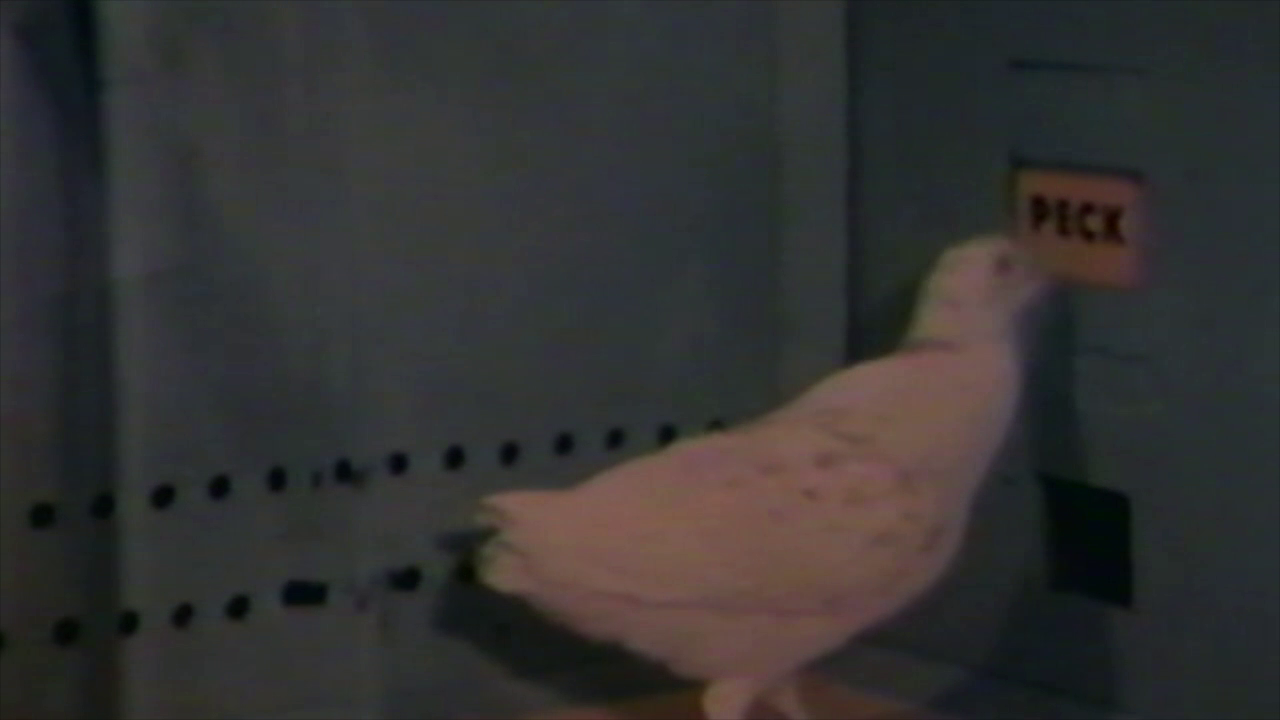
\includegraphics[width=0.45\linewidth]{media/pigeon-peck.png}%
  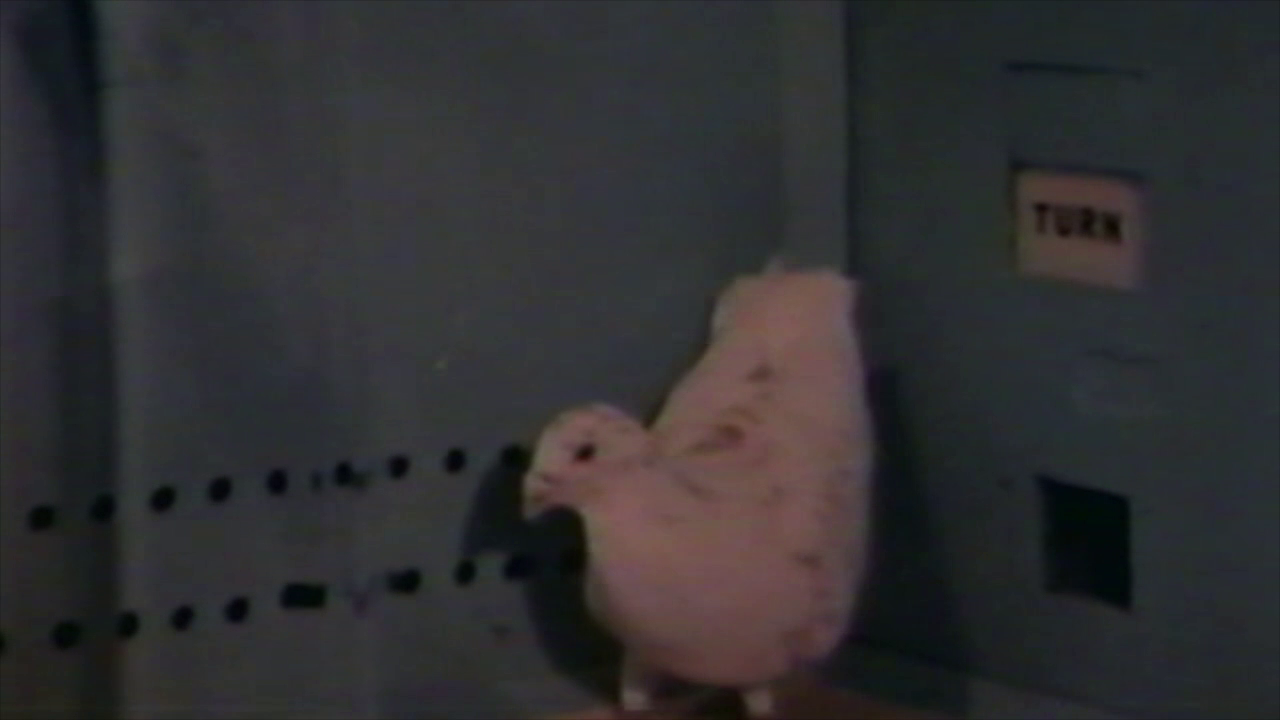
\includegraphics[width=0.45\linewidth]{media/pigeon-turn.png}
  \footnote{Image source:bfskinner.org}

\end{frame}

\note{
  \begin{enumerate}
  \item BF Skinner demonstrated that pigeons could learn to repeat an action
    that lead them to a particular reward.
    \cite[p15]{sutton2020reinforcement}
  \end{enumerate}
}

\begin{frame}{RL terminology}
  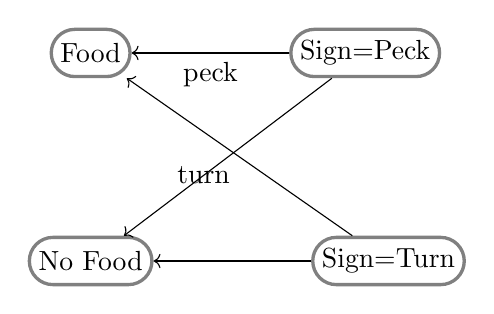
\begin{tikzpicture}[node distance=20mm,
    state/.style={
      % The shape:
      rectangle,minimum size=6mm,rounded corners=3mm,
      % Border
      very thick,draw=black!50
      }]
  \node (food) [state] {Food};
  \node (no-food) [state, below=of food] {No Food};
  \node (sign-peck) [state,right=of food] {Sign=Peck};
  \node (sign-turn) [state,right=of no-food] {Sign=Turn};
  \draw [->] (sign-peck) to [edge label=peck] (food);
  \draw [->] (sign-peck) to (no-food);
  \draw [->] (sign-turn) to [edge label=turn] (food);
  \draw [->] (sign-turn) to (no-food);
  \end{tikzpicture}
  \begin{description}
  \item[State ] ($\bfs_t \in \calS$) Example: Sign is peck or turn. Food is
    dispensed or not.
  \item[Reward function ] ($r_t(\bfs_t) \to \bbR$) Example: Food is high reward ($r_t = 100$).
food is zero-reward ($r_t = 0$).
\item[Actions ] ($\bfa_t \in \calA$) Example: To peck or to turn or no action.
  \item[Transition probabilities]
    ($T(\bfs_{t+1}|\bfs_{t}, \bfa_t) \to [0, 1 ] $) Example:
    Probability of food dispensing if you peck when Sign-peck is shown.
  \end{description}
\end{frame}
\note{
  State is the full description of the world at time $t$ that captures the
entire history. Example: in this example the state can be captured with two bits
$\bfs_t = [f_t; p_t]$, where $f_t \in \{0, 1\}$ describes a food or no food
state and $p_t \in \{0, 1\}$ describes the sign showing  peck or turn.
}

\begin{frame}{Better state diagram}
  \begin{tikzpicture}[node distance=20mm,
    state/.style={
      % The shape:
      rectangle,minimum size=6mm,rounded corners=3mm,
      % Border
      very thick,draw=black!50
    },
    every to/.style={
      thick,bend right
    }
    ]
    \node (food-turn) [state] {Food/Sign=Turn};
    \node (food-peck) [state, below=of food] {Food/Sign=Peck};
    \node (no-food-turn) [state,right=of food] {NoFood/Sign=Turn};
    \node (no-food-peck) [state,right=of no-food] {NoFood/Sign=Peck};
    \draw [-Stealth](no-food-turn) to [edge label=turn] (food-turn);
    \draw [-Stealth](no-food-peck) to [edge label=peck] (food-peck);
    \draw [-Stealth](food-turn) to [edge label=eat] (no-food-turn);
    \draw [-Stealth](food-peck) to [edge label=eat] (no-food-peck);
    \draw [-Stealth](no-food-turn) to [edge label=?] (no-food-peck);
    \draw [-Stealth](no-food-peck) to [edge label=?] (no-food-turn);
    \draw [-Stealth] (no-food-turn.north) to [in=45,out=-45,loop,edge label'=peck] (no-food-turn.north);

    \draw [-Stealth] (no-food-peck.south) to [in=135,out=-135,loop,edge label=turn] (no-food-peck.south);
  \end{tikzpicture}
  
\end{frame}

\begin{frame}{RL problem}
  \begin{description}
      \item[Policy function] 
        $\pi(\bfs_t) \to \bfa_t$\\
      \item[Discount factor ] $\gamma \in (0,1)$.
  \end{description}
  \begin{align*}
    \pi^*(.) = \arg~\max_{\pi} \bbE_{T}\left[\sum_{t=0}^{\infty}
      \gamma^{t} r(\bfs_t) \right]
    \\
    \text{such that } \bfs_{t+1}\sim T(.|\bfs_t, \pi(\bfs_t))\forall t \in [k, \infty) \\
    \text{ and } \bfs_0 \sim p_0(.) 
  \end{align*}
\end{frame}

\begin{frame}{Value Function}
  \begin{align*}
    \pi^*(.) &= \arg~\max_{\pi} \bbE_{T}\left[\sum_{t=0}^{\infty}
    \gamma^{t} r(\bfs_t) \right]
    \\
    \text{such that }& \bfs_{t+1}\sim T(.|\bfs_t, \pi(\bfs_t)) \forall t \in [k, \infty)\\
    \text{ and }& \bfs_0 \sim p_0(.) 
  \end{align*}

  \begin{align*}
    V_\pi(\bfs_k) &= \bbE_{T}\left[\sum_{t=k}^{\infty}
    \gamma^{t} r(\bfs_t) \right]
    \\
    \text{such that }& \bfs_{t+1}\sim T(.|\bfs_t, \pi(\bfs_t)) \forall t \in [k, \infty)\\
  \end{align*}
\end{frame}

\begin{frame}{Action Value Function}
  \begin{align*}
    Q_\pi(\bfs_k, \bfa_k) &= \bbE_{T}\left[\sum_{t=k+1}^{\infty}
                    \gamma^{t} r(\bfs_t) \right]
    \\
    \text{such that }& \bfs_{t+1}\sim T(.|\bfs_t, \pi(\bfs_t)) \forall t \in [k, \infty) \\
  \end{align*}
\end{frame}


\begin{frame}{References}
\bibliography{main}
\bibliographystyle{abbrev}
\end{frame}
\end{document}
